
\section{Applications :}
La vision par ordinateur est appliqué dans nombreux domaines :
\subsection{La santé :}
Les maladies comme la tumeur au cerveau, la maladie de Parkinson, le cancer du sein, le diabète et d’autres sont diagnostiquées à l’aide des ordinateurs et des machines, qui  sont capables de donner un diagnostic précoce d’une maladie plausible, permettant ainsi un traitement à un stade prématuré de la maladie.\\

\begin{center}
    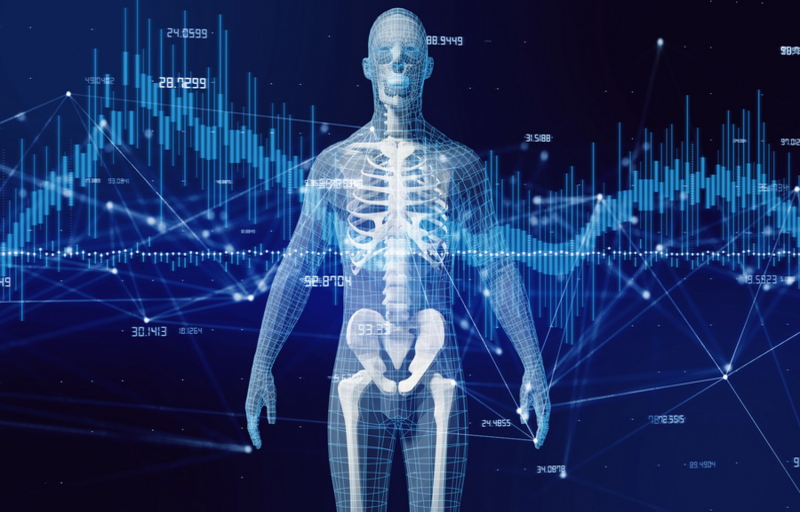
\includegraphics[scale=0.25]{img3.png}
        \captionof{figure}{Une équipe du MIT a conçu un algorithme d’imagerie médicale 3D accélère avec les réseaux de neurones}
        \label{fig1}
\end{center} 

\subsection{Les automobiles :}
Les voitures autonomes d’aujourd’hui qui inclut la détection des collisions, des obstacles et des piétons, elles  peuvent aussi  surveille la bonne conduite d’un conducteur, ainsi réduire les risques d’accidents.\\
\begin{center}
    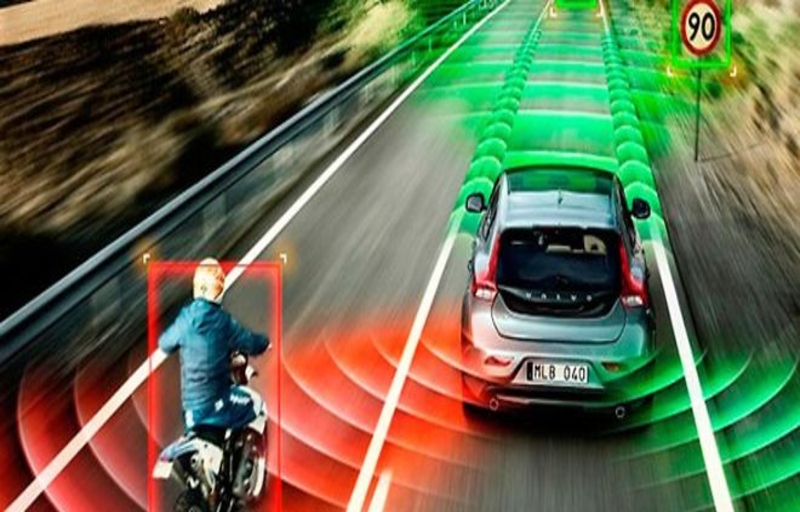
\includegraphics[scale=0.25]{img4.png}
    \captionof{figure}{source: www.lepoint.fr}
    \label{fig2}
\end{center} 
\subsection{La surveillance :}
Un système de sécurité digne de ce nom dispose de caméras permet de donner une surveillance constante de nos écoles scolaires,  stations de métro,  hôpitaux  et n’importe quelle bâtiment nécessitant une surveillance est capable de détecter des crimes tels que le vol, l'intrusion et la violence et détecte aussi les auteurs de crime grâce à la reconnaissance faciale.\\
\begin{center}
    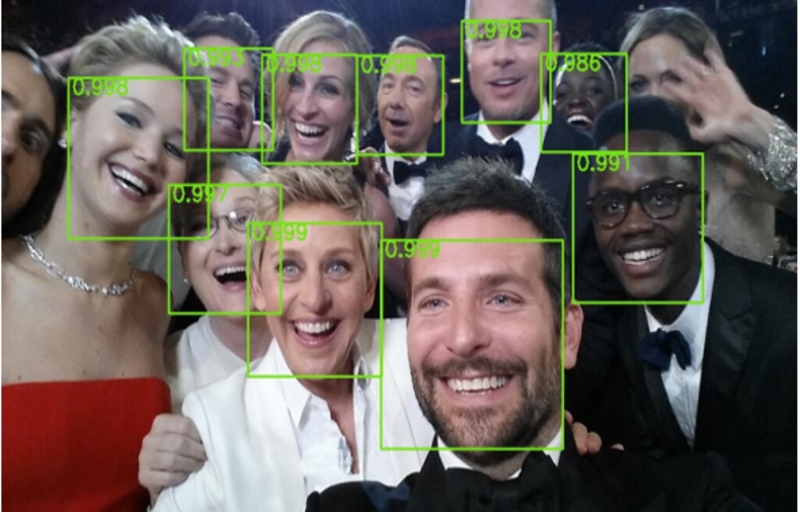
\includegraphics[scale=0.25]{img5.png}
    \captionof{figure}{L'image représente le  résultat des algorithme reconnaissance faciale par www.wikipedia.fr}
    \label{fig2}
\end{center} 
\subsection{L’astronomie :}
Tous les données volumineuses collectées sur notre univers obtenus à l’aide d’ordinateur et satellite, qui nous permet d’étudier ces données rapidement, et découvrir de nouvelles planètes et corps célestes.

\begin{center}
    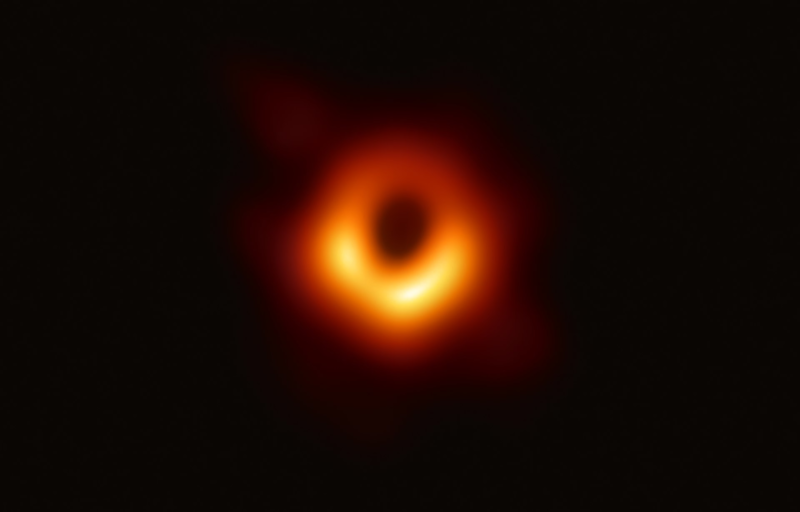
\includegraphics[scale=0.25]{img6.png}
    \captionof{figure}{Images du trou noir supermassif M87 et de son disque d'accrétion par l'Event Horizon Telescope.}
    \label{fig3}
\end{center} 

\subsection{L’agriculture :}
la vision par ordinateur détermine la bonne santé des cultures, identifier les zones fertiles et vérifier la présence de masses d’eau. Elle permet également aux robots de mener des taches tels que la récolte, la plantation et  le désherbage, etc...\\

\subsection{L’industriel :}
Les chaînes de montage comptent les lots, détecte les produits endommagés, détectent les produits avec défauts et dans les tâches de fabrication en général.\\

\begin{center}
    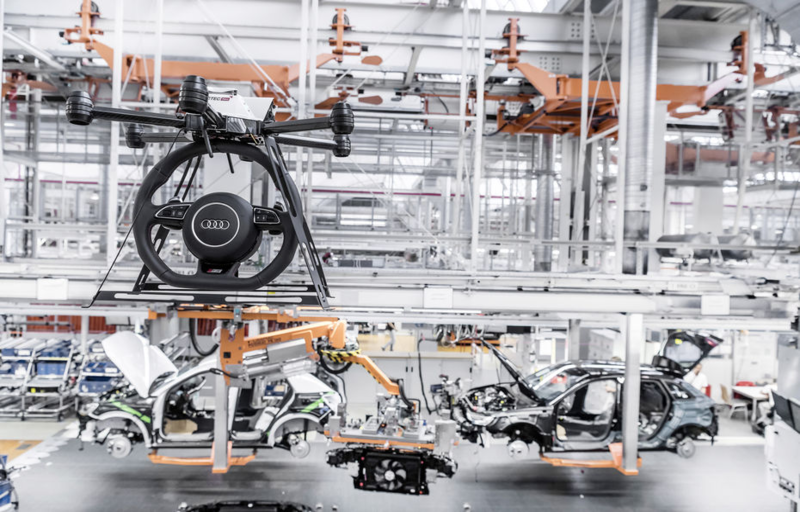
\includegraphics[scale=0.25]{img7.png}
    \captionof{figure}{Drone dans la chaine de montage de voitures de l’usine Audi de Neckarsulm en Allemagne. STEFAN WARTER}
    \label{fig4}
\end{center} 

\subsection{L’imagerie par satellite :}
Les images par satellite détectent les catastrophes naturels telles que les tsunamis, les ouragans et les glissements de terrain, elles permettent aussi d’analyser la pollution et l’indice de la qualité de l’air des zones de concentration. Elles sont utilisées pour vérifier la présence de minerais dans des mines.\\[2cm]

Après  cette introduction sur la vision par ordinateur et ses applications, je vais parler sur certains des algorithmes utilisés en vision par ordinateur.
